\documentclass{article}
\usepackage{minted}
\usepackage{graphicx} % Required for inserting images
\usepackage[UTF8]{ctex}
\usepackage{amsmath}
\usepackage{xcolor} % to access the named colour LightGray
\definecolor{LightGray}{gray}{0.9}

\usepackage[T1]{fontenc}
\usepackage[utf8]{inputenc}
\usepackage{authblk}

\title{软件设计与开发实习报告}

\author[*]{2106050119包涵}
\author[*]{2106050127梁子杰}
\author[*]{2106050128朱轩宇}
\author[*]{2106050129杨磊}
\author[*]{2106050130徐圣翔}
\affil[*]{河海大学信息学部计算机与信息学院软件工程系}
 
\renewcommand\Authands{ and }

\date{\today}

\begin{document}

\maketitle
\begin{figure}[H]
    \centering
    
\includegraphics[scale=0.8]{pircture/xiaohui.png}
\end{figure}


\newpage
\tableofcontents
\newpage

\section{前言}
谣言在社交媒体和网络传播中普遍存在,对个人和社会都造成了负面影响。谣言往往以虚假的信息形式传播,容易误导公众,破坏社会秩序,甚至对个人的声誉和隐私造成伤害。谣言还可能引发恐慌、仇恨和社会不稳定等问题,对社会和国家的发展产生负面影响。

因此,谣言检测变得尤为重要。谣言检测模型的目的是通过分析文本内容、社交媒体数据和其他相关信息,准确判断一个消息是否属于谣言。这些模型可以帮助人们识别和辨别谣言,提供准确的信息,避免被误导和误解。

谣言检测模型的研究和应用具有重要的意义。首先,它可以帮助个人和社会更好地应对谣言的挑战,提高信息的可信度和准确性。其次,谣言检测模型可以为政府、媒体和其他组织提供决策支持,帮助他们更好地管理和应对谣言传播的风险。此外,谣言检测模型还可以为社交媒体平台和互联网公司提供技术支持,帮助他们更好地管理和过滤谣言内容,维护网络环境的健康和秩序。

本次实践课程的课程设计项目,以双向长短期记忆网络(BiLSTM)为基础进行谣言检测模型的开发,BiLSTM模型结合了长短期记忆网络和双向循环神经网络的优点,能够捕捉文本中的语义和上下文信息,从而实现准确的谣言检测。用户无需下载或安装额外的软件,只需在网页上访问该谣言检测软件,即可使用其强大功能。软件使用的灵活性使用户可以在任何时候、任何地点使用该软件进行谣言检测。

这次项目不仅能够让我们将理论课学习的知识应用于实践,更珍贵的是能够让我们了解在团队中一边磨合一边合作的流程,在这一路上所遇到的问题都是对我们团队合作能力的考验。但经过这次实践,我们的团队合作能力也会得到很大提升。

\newpage

\section{概述}
\subsection{项目背景}
社交媒体的发展在加速信息传播的同时,也带来了虚假谣言信息的泛滥,往往会引发诸多不安定因素,并对经济和社会产生巨大的影响。

2016年美国总统大选期间,受访选民平均每人每天接触到4篇虚假新闻,虚假新闻被认为影响了2016年美国大选和英国脱欧的投票结果;近期,在新型冠状病毒感染的肺炎疫情防控的关键期,在全国人民都为疫情揪心时,网上各种有关疫情防控的谣言接连不断,从“广州公交线路因新型冠状病毒肺炎疫情停运”到“北京市为防控疫情采取封城措施”,从“钟南山院士被感染”到“10万人感染肺炎”等等,这些不切实际的谣言,“操纵”了舆论感情,误导了公众的判断,更影响了社会稳定。

\subsection{编写目的}
人们常说“流言止于智者”,要想不被网上的流言和谣言盅惑、伤害,首先需要对其进行科学甄别,而时下人工智能正在尝试担任这一角色。那么,在打假一线AI技术如何做到去伪存真?

传统的谣言检测模型一般根据谣言的内容、用户属性、传播方式人工地构造特征,而人工构建特征存在考虑片面、浪费人力等现象。本次实践使用基于长短期记忆神经网络(BiLSTM)的谣言检测模型,将文本中的谣言事件向量化,通过循环神经网络的学习训练来挖掘表示文本深层的特征,避免了特征构建的问题,并能发现那些不容易被人发现的特征,从而产生更好的效果。

\subsection{软件定义}
本次课程设计基于双向长短期记忆网络(BiLSTM)为基础进行谣言检测模型的开发,该模型通过分析文本内容、社交媒体数据和其他相关信息,准确判断一个消息是否属于谣言。用户无需下载或安装额外的软件,只需在网页上访问该谣言检测软件,即可使用其强大功能。软件使用的灵活性使用户可以在任何时候、任何地点使用该软件进行谣言检测。软件会根据输入的文本进行实时检测,并将结果直观地展示给用户。并且会展示本软件中搜索量最高的话题,清晰地向用户展现热点谣言和舆论趋势。

\subsection{开发环境}
后端开发环境为:
\begin{itemize}
  \item [1)]
  Django 4.2.2
  \item [2)]
  Pycharm 2022.1.3
  \item [3)]
  Python 3.11
  \item [4)]
  PyMySQL 1.1.0
\end{itemize}

前端开发环境为:
\begin{itemize}
  \item [1)]    Vue 3.3.4
  \item [2)]    Vite
  \item [3)]    echarts 5.4.2
  \item [4)]    ant-design 1.0.0
  \item [5)]    axios 9.5.1
\end{itemize}

算法开发环境为:
\begin{itemize}
  \item [1)]
  conda 22.9.0
  \item [2)]
  pytorch 2.0.1
\end{itemize}

部署环境:
\begin{itemize}
  \item [1)]
  操作系统 Ubuntu Server 22.04 LTS 64bit
  \item [2)]
  MySQL 8.0.32-0ubuntu0.22.04.2
  \item [3)]
  CPU-2核,内存-2GB,系统盘-SSD云硬盘40GB腾讯云服务器
\end{itemize}

\newpage

\section{系统需求分析}
\subsection{选题陈述}
当前谣言检测存在一些问题。首先,谣言检测的准确性还有待提高。由于谣言的形式多样,包括文字、图片、视频等,而且谣言制造者也在不断改进其制造技巧,使得谣言检测变得更加困难。其次,谣言检测的速度需要进一步提高。随着信息传播的速度越来越快,谣言往往在短时间内迅速传播,而谣言检测的过程需要一定的时间,导致谣言可能已经在社交网络中广泛传播了。此外,谣言检测还面临着大规模数据处理和信息过滤的挑战,需要处理大量的信息并筛选出可能的谣言。最后,谣言检测还需要解决隐私和伦理问题。在进行谣言检测时,可能需要获取用户的个人信息和社交网络数据,这涉及到隐私保护和数据使用的伦理问题。

所以,我们想通过以双向长短期记忆网络(BILSTM)为基础开发一个谣言检测模型,进行大规模的数据处理,来提高谣言检测的速度和准确性。

\subsection{需完成的功能}
\begin{itemize}
  \item [1)]    谣言检测功能:要准确判断谣言,模型应能够准确地判断一个消息是否属于谣言,避免误判和漏判。
  \item [2)]    谣言热度榜功能:实现对谣言数据的增删改查以及谣言榜单查询的相关功能。
\end{itemize}

\subsection{数据流图}

\begin{figure}[H]
    \centering
    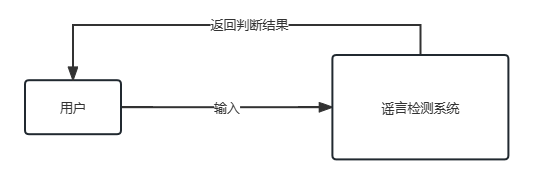
\includegraphics[scale=0.6]{pircture/数据流图.png}
\end{figure}

\subsection{数据表}
\begin{figure}[H]
    \centering
    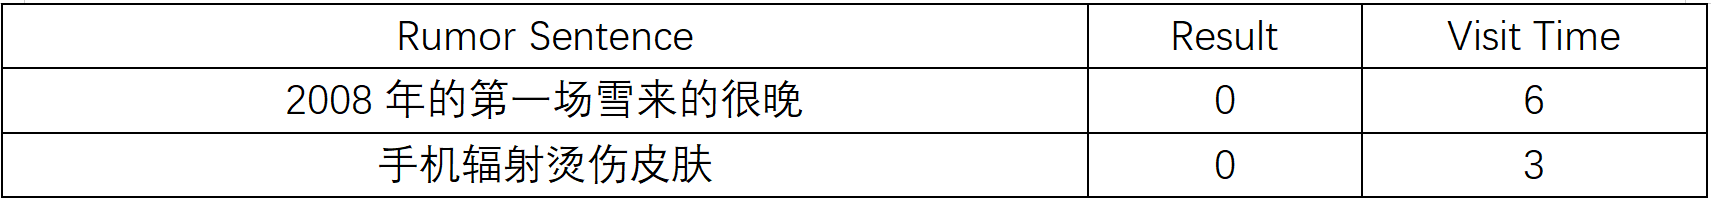
\includegraphics[scale=0.2]{pircture/数据表.png}
\end{figure}

数据库中存放一张表来实现谣言点击热度榜的功能,并实现快速返回结果的功能,表名为RumorList。

表中共有3个字段,RumorSentence字段类型为VARCHAR,长度为100,用于存储用户输入的每条谣言内容;Result字段类型为int,用于存储深度学习模型处理后的结果,字段为0表示不是谣言,字段为1表示是谣言;VisitTime字段类型为int,用于存储所有用户对该谣言的访问次数,当用户访问时,先查询RumorList表中是否存在相同的谣言,如果存在则直接返回结果,不存在则把VisitTime字段初始化为1,当用户访问点击热度榜时,对表根据VisitTime和主键两个因素从大到小排序并取出前10条记录,从而实现谣言点击热度榜功能。

本项目的MySQL数据库部署在Linux服务器上,通过远程连接的方式操作。

\newpage

\section{算法总体流程设计}
调用双向长短期记忆网络模块,将谣言内容输入模型内部,通过双向长短期记忆网络中的多个LSTM单元,捕捉谣言内容序列中的前后依赖关系,输出结果最终实现谣言检测功能。

双向长短期记忆网络(Bidirectional LSTM)是一种循环神经网络(Recurrent Neural Network, RNN)的变体,用于处理序列数据。与传统的单向 LSTM 不同,双向 LSTM 在每个时间步上都有两个 LSTM 单元,分别按正向和反向顺序处理输入序列。它能够捕捉到序列数据中前后依赖关系的特征,从而更好地理解和表示序列数据。

\begin{itemize}
  \item [1)]
  输入序列:首先,将输入序列按时间步拆分为一个个单词或符号,并将其作为 LSTM 的输入。
  \item [2)]
  正向传播:正向 LSTM 单元按照时间步的顺序逐个处理输入序列。在每个时间步,正向 LSTM 单元接收当前时间步的输入和前一时间步的隐藏状态,并计算当前时间步的输出和隐藏状态。输出可以是当前时间步的隐藏状态、当前时间步的预测结果或其他自定义的输出。
  \item [3)]
  反向传播:反向 LSTM 单元按照时间步的逆序逐个处理输入序列。在每个时间步,反向 LSTM 单元接收当前时间步的输入和后一时间步的隐藏状态,并计算当前时间步的输出和隐藏状态。
  \item [4)]
  合并结果:正向 LSTM 和反向 LSTM 的输出在每个时间步上都有一个值,可以将这两个值按时间步进行连接或合并,形成一个更丰富的表示。
  \item [5)]
  输出结果:可以使用合并结果进行进一步的处理,如添加额外的全连接层、进行分类、回归或其他任务。
\end{itemize}

双向 LSTM 的优点在于它能够同时考虑到过去和未来的信息,捕捉到输入序列中的长期依赖关系。它通过正向和反向传播的结合,可以在每个时间步上利用过去和未来的上下文信息,从而更好地建模序列数据。在文本分类、情感分析、命名实体识别等自然语言处理任务中,双向 LSTM 常被应用于对输入文本的建模,能够有效地捕捉上下文信息,提升模型的性能和表达能力。

\newpage

\section{软件功能设计}
\begin{figure}[H]
    \centering
    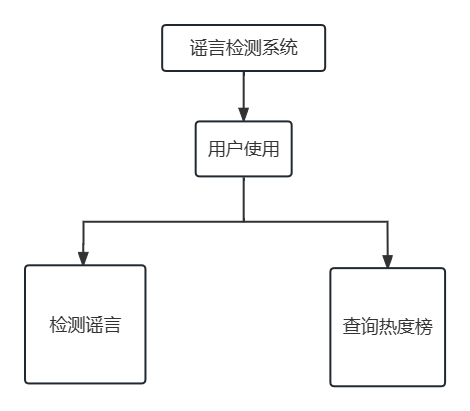
\includegraphics[scale=0.6]{pircture/软件功能设计.png}
\end{figure}

检测谣言:主要实现将用户查询的语句传到后端,调用谣言检测模块得出判断结果,并返回前端并显示结果。

查询热度榜:主要和数据库有关,数据库存储用户每一次的查询的内容和其查询的次数,实现将数据库中查询次数最高的10个谣言展示到前端热度榜。

\newpage

\section{算法模型代码设计}
模块1:从两个目录(true\_dir和fake\_dir)中读取JSON文件,并将文件中的文本数据提取出来。

然后将文本数据分为训练集和测试集,并将它们分别写入到"train.txt"和"test.txt"两个文件中。 该部分代码的主要功能是将两个目录中的JSON文件提取出文本数据,并将其划分为训练集和测试集,然后将数据写入到两个文本文件中。这些文本文件可以作为机器学习模型的输入数据,用于进行文本分类或其他相关任务。
\begin{minted}
[
frame=lines,
framesep=2mm,
baselinestretch=1.2,
bgcolor=LightGray,
fontsize=\footnotesize,
linenos
]
{Python}
def get_train_val_txt(true_dir="non-rumor-repost", fake_dir="rumor-repost"):
    datasets, labels = [], []
    for i, json_dir in enumerate([true_dir, fake_dir]):
        for json_name in tqdm(os.listdir(json_dir)):
            json_path = json_dir + "/" + json_name
            f = open(json_path, encoding="utf-8")
            json_list = json.load(f)
            for json_obj in json_list:
                text = json_obj.get("text", "")
                text = text.strip().replace("\n", "").replace("[", "").
                    replace("]", "").replace("…", "").replace("@", "")
                if len(text) > 10:
                    datasets.append(text)
                    labels.append(i)
            f.close()
    datasets_train, datasets_test, labels_train, labels_test = 
        train_test_split(datasets, labels, train_size=0.8,shuffle=True)
    with open("train.txt", "w", encoding="utf-8") as f1, open("test.txt", "w", 
        encoding="utf-8") as f2:
        for i in range(len(datasets_train)):
            f1.write(datasets_train[i] + "\t" + str(labels_train[i]) + "\n")
        for i in range(len(datasets_test)):
            f2.write(datasets_test[i] + "\t" + str(labels_test[i]) + "\n")
\end{minted}

模块2:构建一个单词字典,用于将单词映射为索引。该代码的主要功能是从给定的文件中统计单词出现的次数,并构建一个单词字典,将常见的单词映射为索引。 这个字典可以用于将文本数据转换为数字序列,以便在机器学习模型中进行处理。

\begin{minted}
[
frame=lines,
framesep=2mm,
baselinestretch=1.2,
bgcolor=LightGray,
fontsize=\footnotesize,
linenos
]
{Python}
def get_word_dict(root1="train.txt", root2="test.txt", n_common=3000):
    word_count = Counter()
    for root in [root1, root2]:
        with open(root, "r", encoding="utf-8") as f:
            for line in f.readlines():
                line_split = line.strip().split("\t")
                for word in line_split[0]:
                    word_count[word] += 1
    most_common = word_count.most_common(n_common)
    word2index_dict = {word: index + 2 for index, (word, count) 
                       in enumerate(most_common)}
    word2index_dict["UNK"] = 1
    word2index_dict["PAD"] = 0
    return word2index_dict
\end{minted}

模块3:定义了一个名为DataGenerator的数据集类,用于生成训练或测试数据。

继承自Dataset类,通过重写\_\_init\_\_、\_\_getitem\_\_、\_\_len\_\_等方法来实现数据集的功能。该部分代码定义了一个数据集类DataGenerator,该类从文件中读取数据集和标签,并在需要时对数据进行填充或截断。通过使用这个数据集类,可以方便地生成适用于训练或测试的数据样本。

\begin{minted}
[
frame=lines,
framesep=2mm,
baselinestretch=1.2,
bgcolor=LightGray,
fontsize=\footnotesize,
linenos
]
{Python}
class DataGenerator(Dataset):
    def __init__(self, word2index_dict, root="train.txt", max_len=50):
        super(DataGenerator, self).__init__()
        self.root = root
        self.max_len = max_len
        self.word2index_dict = word2index_dict
        self.datasets, self.labels = self.get_datasets()

    def __getitem__(self, item):
        dataset = self.datasets[item]
        label = self.labels[item]
        if len(dataset) < self.max_len:
            dataset += [0] * (self.max_len - len(dataset))
        else:
            dataset = dataset[:self.max_len]
        return torch.LongTensor(dataset), torch.from_numpy(np.array(label)).long()

    def __len__(self):
        return len(self.labels)

    def get_datasets(self):
        datasets, labels = [], []
        with open(self.root, "r", encoding="utf-8") as f:
            for line in f.readlines():
                line_split = line.strip().split("\t")
                datasets.append([self.word2index_dict.get(word, 1) 
                        for word in list(line_split[0])])
                labels.append(int(line_split[1]))
        return datasets, labels
\end{minted}

模块4:定义了一个名为BiLSTMModel的双向LSTM模型类,用于文本分类任务。该模型继承自nn.Module类,通过重写\_\_init\_\_和forward方法来定义模型的结构和前向计算过程。
该模型接收词索引作为输入,经过嵌入层和双向LSTM层的处理,最终输出分类结果的分数。

\begin{minted}
[
frame=lines,
framesep=2mm,
baselinestretch=1.2,
bgcolor=LightGray,
fontsize=\footnotesize,
linenos
]
{Python}
class BiLSTMModel(nn.Module):

    def __init__(self, num_vocab):
        super(BiLSTMModel, self).__init__()
        self.embedding = nn.Embedding(num_embeddings=num_vocab, embedding_dim=128)
        self.lstm = nn.LSTM(input_size=128, hidden_size=256, bidirectional=True, 
                    batch_first=True, num_layers=2)
        self.fc1 = nn.Sequential(
            nn.Linear(512, 512),
            nn.ReLU(inplace=True)
        )
        self.fc2 = nn.Linear(512, 2)

    def forward(self, x):
        out = self.embedding(x)
        outputs, (h, c) = self.lstm(out)
        out = torch.cat([h[-1, :, :], h[-2, :, :]], dim=-1)
        out = self.fc1(out)
        return self.fc2(out)
\end{minted}

模块5:该代码主要实现了一个训练函数train(),用于训练BiLSTM Model模型并输出训练过程中的准确率和测试准确率。该代码实现了一个完整的训练过程,包括模型的初始化、数据加载、模型训练、测试和保存模型等步骤。在训练过程中,每个epoch会输出训练准确率和测试准确率,并在每10个epoch时保存模型。

\begin{minted}
[
frame=lines,
framesep=2mm,
baselinestretch=1.2,
bgcolor=LightGray,
fontsize=\footnotesize,
linenos
]
{Python}
def train():
    device = torch.device("cuda")
    word2index_dict = get_word_dict()
    model = BiLSTMModel(len(word2index_dict)).to(device)
    optimizer = optim.Adam(model.parameters(), lr=1e-3)
    schedule = optim.lr_scheduler.StepLR(optimizer, step_size=2000, gamma=0.9)
    loss_func = nn.CrossEntropyLoss()
    train_loader = DataLoader(DataGenerator(word2index_dict, root="train.txt"), 
                   shuffle=True, batch_size=64)
    test_loader = DataLoader(DataGenerator(word2index_dict, root="test.txt"), 
                   shuffle=False, batch_size=64)
    for epoch in range(31):
        train_accuracy = train_one_epoch(model, train_loader, loss_func, 
                         optimizer, schedule, device, epoch)
        test_accuracy = get_test_result(model, test_loader, device)
        print(f"epoch:{epoch + 1},train accuracy:{train_accuracy},
                test accuracy:{test_accuracy}")
        if (epoch + 1) % 10 == 0:
            torch.save(model, f"bilstm_model_epoch{epoch + 1}.pth")
\end{minted}

模块6:该代码主要实现了一个函数`train\_one\_epoch(),用于对模型进行一轮训练,并返回训练准确率。该代码实现了模型的一轮训练过程,包括将模型设置为训练模式、遍历训练数据集、计算损失、更新模型参数、更新学习率和计算训练准确率等步骤。在每个批次的训练中,会输出当前的训练损失和学习率,并在最后返回训练准确率。

\begin{minted}
[
frame=lines,
framesep=2mm,
baselinestretch=1.2,
bgcolor=LightGray,
fontsize=\footnotesize,
linenos
]
{Python}
def train_one_epoch(model, train_loader, loss_func, optimizer, 
        schedule, device, epoch):
    model.train()
    data = tqdm(train_loader)
    labels_true, labels_pred = np.array([]), np.array([])
    for batch, (x, y) in enumerate(data):
        labels_true = np.concatenate([labels_pred, y.numpy()], axis=-1)
        datasets_train, labels_train = x.to(device), y.to(device)
        prob = model(datasets_train)
        pred = torch.argmax(prob, dim=-1).cpu().numpy()
        labels_pred = np.concatenate([labels_pred, pred], axis=-1)
        loss = loss_func(prob, labels_train)
        optimizer.zero_grad()
        loss.backward()
        optimizer.step()
        schedule.step()
        data.set_description_str(
            f"epoch:{epoch + 1},batch:{batch + 1},loss:{loss.item()},
                    lr:{schedule.get_last_lr()[0]}")
    accuracy = np.mean(np.array(labels_pred == labels_true).astype(int))

    return accuracy
\end{minted}

模块7:该代码主要实现了一个函数get\_test\_result(),用于对模型进行测试并输出测试结果。该代码实现了对模型进行测试,并输出测试结果,包括测试准确率、精确率、召回率、F1值、ROC曲线和混淆矩阵。在测试过程中,会将预测结果的概率进行保存,并根据真实标签和预测标签计算各种评估指标,并将ROC曲线和混淆矩阵进行绘制和保存。

\begin{minted}
[
frame=lines,
framesep=2mm,
baselinestretch=1.2,
bgcolor=LightGray,
fontsize=\footnotesize,
linenos
]
{Python}
def get_test_result(model, test_loader, device):
    model.eval()
    data = tqdm(test_loader)
    labels_true, labels_pred = np.array([]), np.array([])
    labels_prob = []
    with torch.no_grad():
        for x, y in data:
            labels_true = np.concatenate([labels_true, y.numpy()], axis=-1)
            datasets_test = x.to(device)
            prob = model(datasets_test)
            pred = torch.argmax(prob, dim=-1).cpu().numpy()
            labels_pred = np.concatenate([labels_pred, pred], axis=-1)
            labels_prob.append(prob.cpu().numpy())
    labels_prob = np.concatenate(labels_prob, axis=0)
    precision = precision_score(labels_true, labels_pred)
    recall = recall_score(labels_true, labels_pred)
    f1 = f1_score(labels_true, labels_pred)
    accuracy = np.mean(np.array(labels_pred == labels_true).astype(int))
    print(f"accuracy:{accuracy},precision:{precision},recall:{recall},f1:{f1}")

    fpr, tpr, _ = roc_curve(labels_true, labels_prob[:, -1])

    plt.figure(figsize=(8, 8))
    plt.plot([0, 1], [0, 1], "r--")
    plt.plot(fpr, tpr, "green", label=f"AUC:{auc(fpr, tpr)}")
    plt.legend()
    plt.title("BiLSTM roc_curve")
    plt.savefig("roc_curve.png")
    matrix = confusion_matrix(labels_true, labels_pred, normalize="true")

    plt.figure(figsize=(8, 8))
    seaborn.heatmap(matrix, annot=True, cmap="GnBu")
    plt.title("confusion_matrix")
    plt.savefig("confusion_matrix.png")

    return accuracy
\end{minted}

通过在测试集上的测试,可以得到模型的准确率为77\%。混淆矩阵和ROC曲线如下:
\maketitle
\begin{figure}[H]
    \centering
    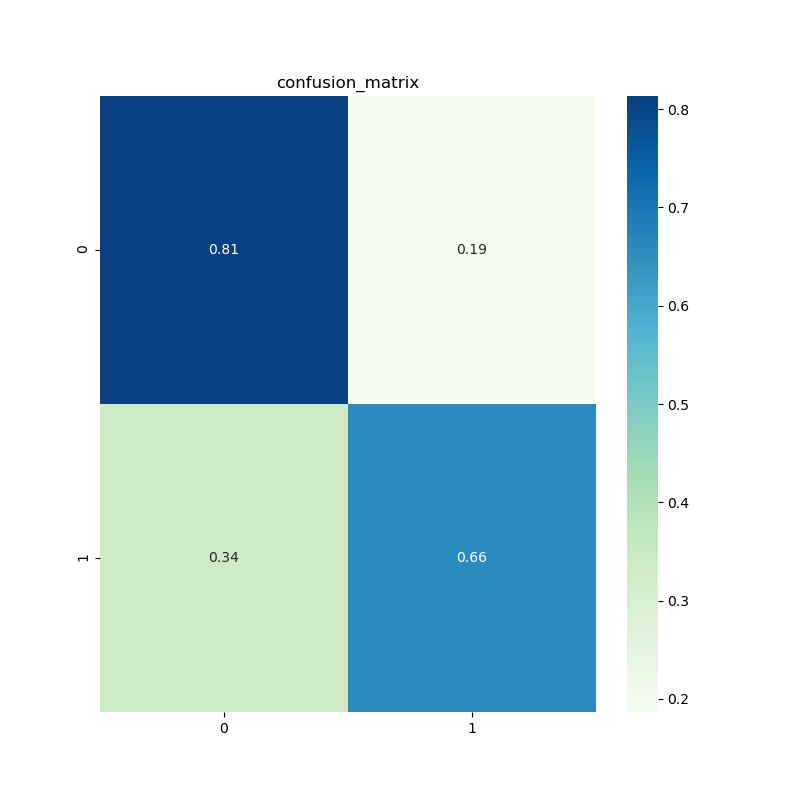
\includegraphics[scale=0.4]{pircture/confusion_matrix.png}
\end{figure}

\maketitle
\begin{figure}[H]
    \centering
    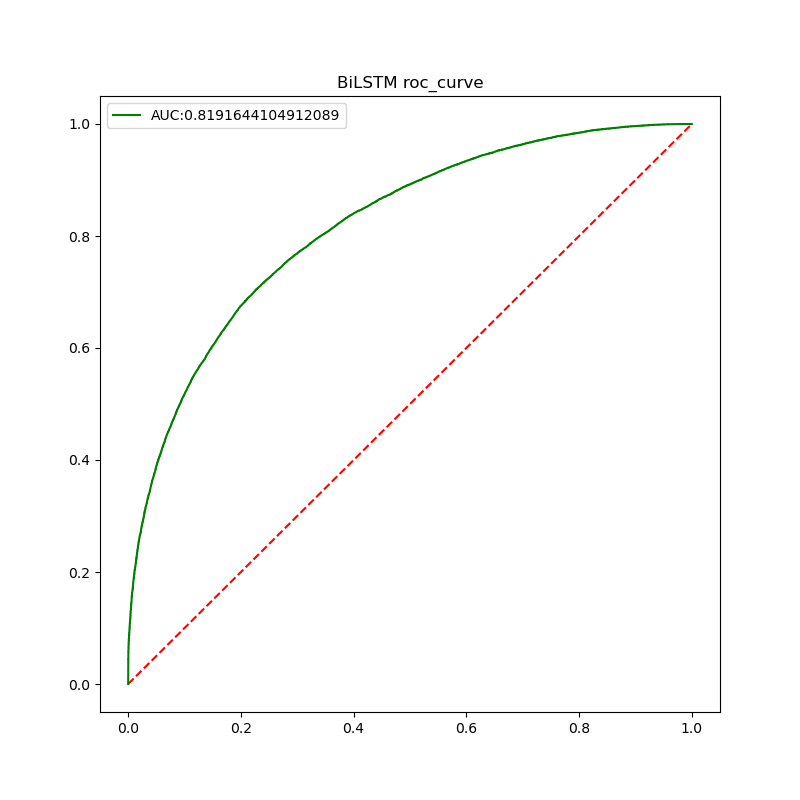
\includegraphics[scale=0.4]{pircture/roc_curve.png}
\end{figure}

模块8:该代码实现了一个函数predict(),用于对输入的句子进行预测并输出预测结果。

考虑到服务器上只有CPU而没有GPU的情况,便采用了在本机GPU训练,再上传到服务器CPU上进行预测的模式。

\begin{minted}
[
frame=lines,
framesep=2mm,
baselinestretch=1.2,
bgcolor=LightGray,
fontsize=\footnotesize,
linenos
]
{Python}
def predict(sentence, model_path="bilstm_model_epoch10.pth"):
    labels = ["真话", "谣言"]
    device = torch.device('cuda' if torch.cuda.is_available() else 'cpu')
    word2index_dict = get_word_dict()
    sentence = [word2index_dict.get(word, 1) for word in sentence]
    if len(sentence) < 50:
        sentence += [0] * (50 - len(sentence))
    else:
        sentence = sentence[:50]
    datasets = torch.unsqueeze(torch.LongTensor(sentence), dim=0).to(device)
    model = torch.load(model_path, map_location = 'cpu')
    model.eval()
    with torch.no_grad():
        labels_pred = torch.argmax(model(datasets), dim=-1).cpu().numpy()[0]
    return labels_pred
\end{minted}

模块9:该部分代码主要实现了一个函数module\_evaluation(),用于加载训练好的模型,并对测试数据进行评估。该代码实现了加载训练好的模型,并在测试数据上进行评估。它首先加载模型,然后使用数据加载器加载测试数据,最后调用get\_test\_result函数计算评估指标并输出结果。

\begin{minted}
[
frame=lines,
framesep=2mm,
baselinestretch=1.2,
bgcolor=LightGray,
fontsize=\footnotesize,
linenos
]
{Python}
def module_evaluation():
    model = torch.load("bilstm_model_epoch10.pth").to("cuda")
    test_loader = DataLoader(DataGenerator(get_word_dict(), root="test.txt"), 
                  shuffle=False, batch_size=64)
    get_test_result(model, test_loader, "cuda")

    return
\end{minted}

\newpage

\section{界面设计}

\begin{figure}[H]
    \centering
    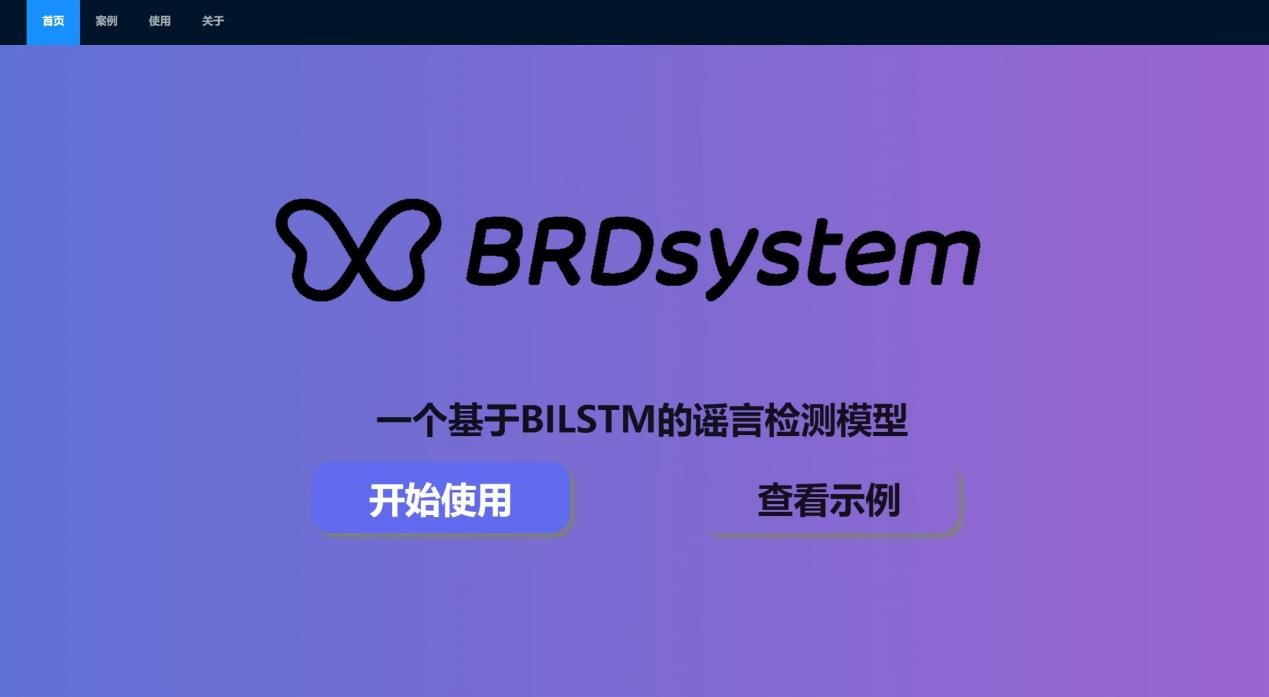
\includegraphics[scale=0.8]{pircture/主界面.jpg}
\end{figure}

网页主界面如上图所示,点击开始使用即可进入如下页面:

\begin{figure}[H]
    \centering
    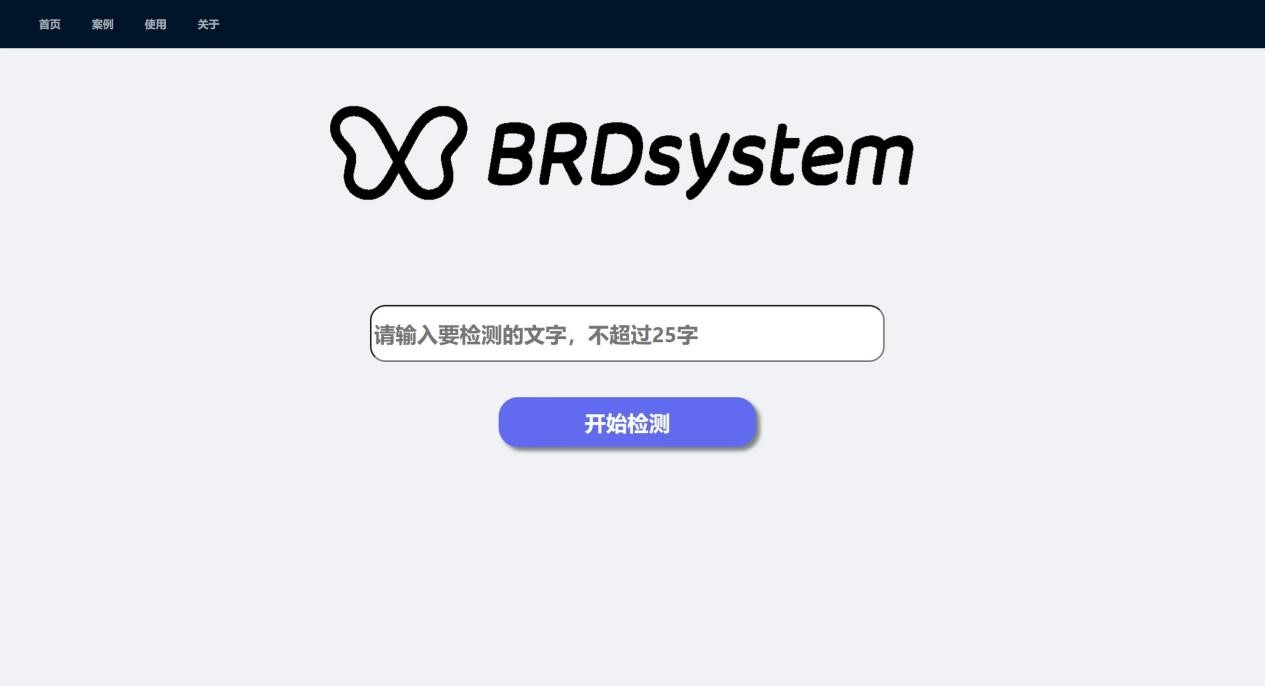
\includegraphics[scale=0.8]{pircture/查询界面.jpg}
\end{figure}

在输入框中输入想检测的话题,再点击开始检测,即可开始检测谣言。

\begin{figure}[H]
    \centering
    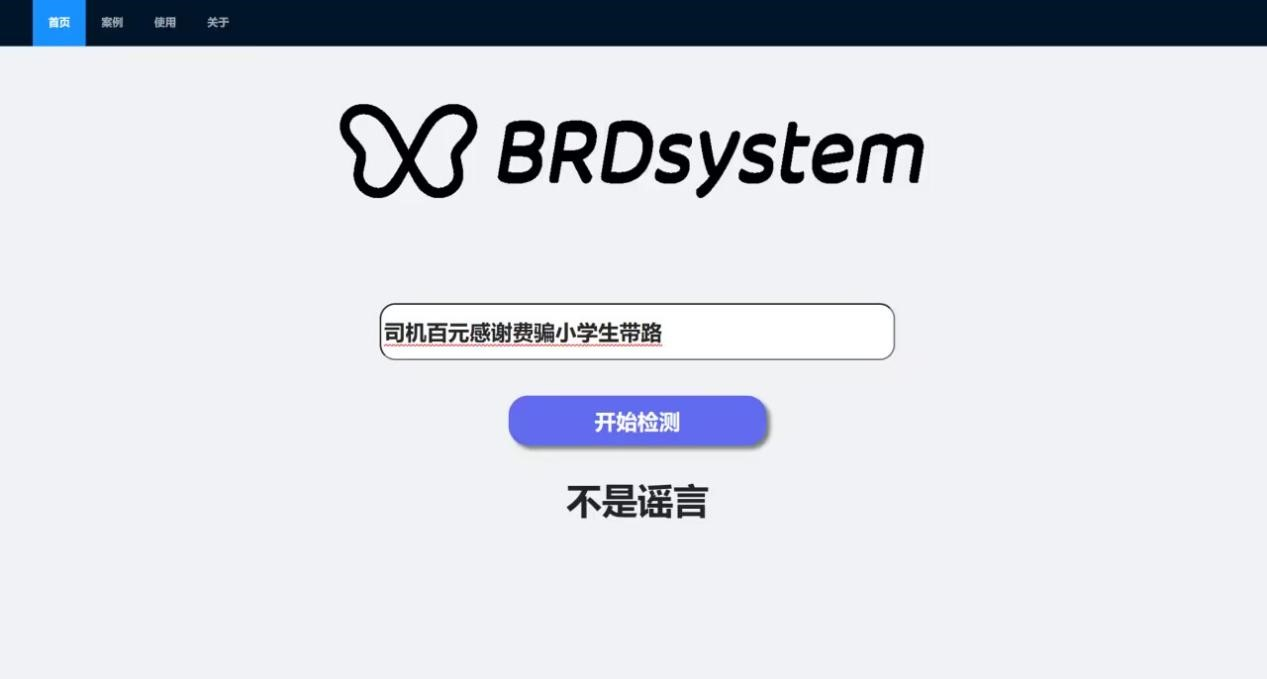
\includegraphics[scale=0.8]{pircture/结果界面.jpg}
\end{figure}

我们的谣言检测模型即可给出判断,将结果显示出来。接着点击案例,即可查看谣言搜索热度榜,榜单上会呈现搜索量前十的话题。

\begin{figure}[H]
    \centering
    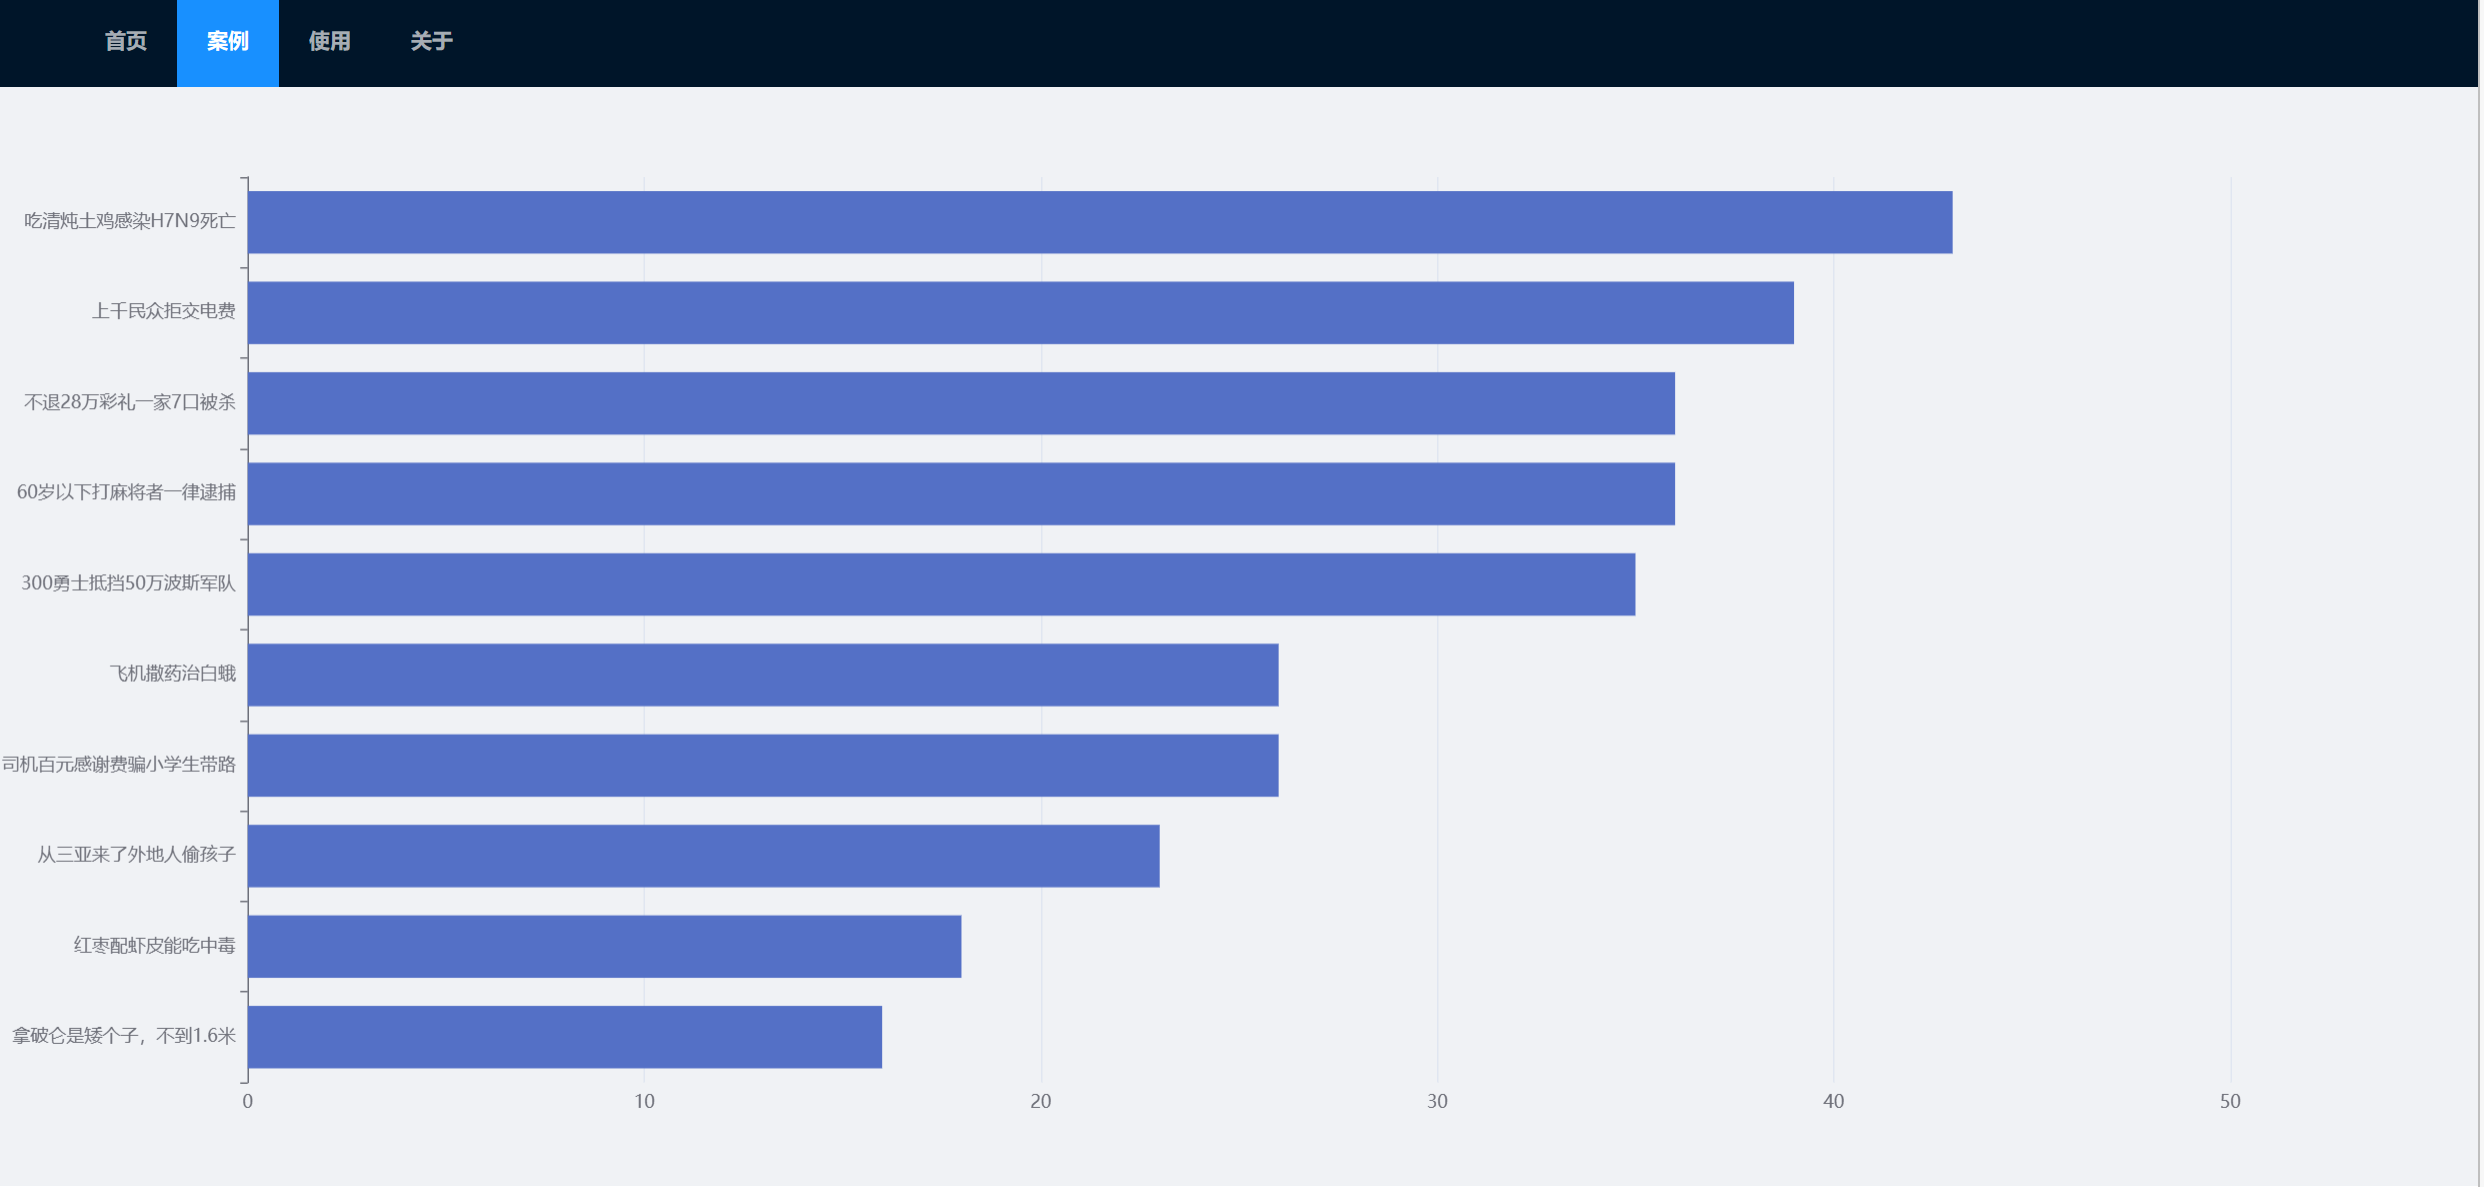
\includegraphics[scale=0.1]{pircture/热度榜界面.png}
\end{figure}

代码存放于Github仓库中,网址为https://github.com/Software-development-design。服务器公网IP为43.143.36.202。

\newpage

\section{小结}
\subsection{小组分工}
徐圣翔:负责实现BiLSTM双向长短期记忆神经网络,实现谣言检测功能,为后端提供接口,同时将前后端部署到Linux服务器上。

包涵:负责前端构建工具构建前端界面,设计UI。

朱轩宇与杨磊:负责用Django构建后端框架,实现和前端的联调。以及后端框架连接机器模型,连接数据库。其中朱轩宇还负责了ppt的制作。

梁子杰:进行代码的汇总和分析,报告编写。

\subsection{遇到的问题}
我们在编写后端代码时遇到了很多问题,但是经过我们小组的集体讨论和debug,我们最终解决了我们遇到的问题。其中遇到的问题如下。
\\

问题1:参数不一致。由于我们小组的后端代码部分不是一个人单独编写的,在代码整合时,试运行报了很多错,经过检查得出,是传递的参数没有完全一致,按理来说这种低级错误是可以避免的,但是由于我们的粗心还是遇到了。关于这个问题的思考,编写代码还是要仔细小心小一点。
\\

问题2:找不到train.txt的路径。在调用核心谣言检测模块时,因为模块是在单独的一个项目中运行的,不存在找不到文件的问题,但在导入我们的实际项目文件的时候,原本用来放置训练数据的文档train.txt会出现在app目录下找不到的情况,导致核心模块无法运行,经过上网查阅这个错误的解决方法,我们尝试了将train.txt的引用路径由相对路径改为绝对路径,虽然这个办法可以解决找不到路径这个问题,但是对于代码来说用绝对路径太繁琐了。最终的解决方法是将train.txt的位置移到项目的根目录下,因为Django框架对外部调用自己写的神经网络模型代码的搜索是优先从根目录开始搜索,所以把文件放根目录就可以解决找不到路径这个问题。
\\

问题3:JSON序列化的问题。在我们接收前端的数据导入谣言检测模型进行判断后,将模型返回的值传到前端时报了Object of type int64 is not JSON serializable的错误。经过网上查阅资料我们得知,当我们使用JSON包返回数据给前端的时候,JSON包需要包装成特殊的格式,因为原谣言检测模块传出的数据是int64型数据,所以我们需要使用JSON包传送格式,也叫字典格式传给前端,该过程叫JSON序列化。字典中包含传给前端的数据名字以及其内容。
\\

问题4:调用的库只兼容python2.x。这个也是上网查阅资料得知,Mysqldb仅支持python 2.x版本,和项目当前使用的django框架不兼容,需要另外进行初始化更改操作,在app目录下的\_init\_.py文件中添加如下代码即可解决问题。

\begin{minted}
[
frame=lines,
framesep=2mm,
baselinestretch=1.2,
bgcolor=LightGray,
fontsize=\footnotesize,
linenos
]
{Python}
import pymysql
pymysql.install_as_MySQLdb()
\end{minted}
\\

问题5:缺少运行环境。核心谣言检测模块需要特殊的运行环境,比如Annaconda环境,Pytorch环境等,因此在没有安装这些环境的电脑上无法运行谣言检测程序,这导致我们中期只能在一台电脑上对文件进行操作,后续只需安装相关环境即可。
\\

问题6:版本控制问题。在我们遇到bug的时候,因为缺少相关经验,我们把其他完好的项目的文件完全复制到了我们的项目文件中,其中的.idea文件夹变化导致PyCharm无法读取我们的文件,并且无法恢复,此前我们在交流软件中传入了能运行的版本,但中间我们修改的版本并没有传入,这导致我们增加了几个小时的工作量,这是一个非常严重的问题。因此我们在后续的所以代码编写中都对代码进行了版本控制,并将能运行的代码传入了Github,进一步完善了我们的代码版本控制。
\\

问题7:与前端对接的问题。这部分问题是我们不熟悉和前端的对接导致的,譬如返回数据包是用GET还是POST方法,前端对接的url的问题,因为这个问题发生时间较早,我们当时不知道我们写的方法是不是有问题,导致了后面其他类型的报错我们也当成了此类问题进行修改,增加了我们的工作时间,在后续的不断学习中,此类问题已经得到改善。
\\

问题8:运行环境版本不兼容。此问题的出现是因为组内成员认为新版本的软件不够稳定,导致组内各成员间软件版本不一致,在后续的代码整合中出现了一个能运行一个不能的问题,并且升级版本等于大部分代码需要重写和调试,这无疑也增加了我们的工作量,在后续的时间中,我们组内做到了版本的统一,问题得以解决。
\\

问题9:Linux的操作和Windows的操作有很大的区别,很不适应。但是不得不说,Linux环境下的开发的确比Windows高效。比如在下载python库的时候,Linux可以无视地域直接快速安装。此外,Linux环境下的开发也比Windows更为高效。当遇到一些问题时,会发现StackOverflow上的解决方法远远多于CSDN。

\subsection{总结}
在短短几天之内,我们学习了各类框架如何使用,时间较短,因此在我们遇到的各类报错中,有很大一部分是我们并不熟悉如何使用这些框架或环境,这让我们意识到实践与理论知识的结合,以及团队间的合作,共同分析等是尤为的重要。

首先,团队合作是这门课程的重点之一。通过一起完成各种项目和任务,我们学会了如何有效地与团队成员合作,分工合作,共同解决问题。在团队合作中,我们学会了倾听他人的意见和建议,学会了尊重和信任团队成员,这对于软件设计的成功非常重要。

其次,这门课程注重理论知识与实践的结合。我们不仅学习了软件设计的理论知识,还通过实践项目来应用这些知识。通过实践,我们更深入地理解了软件设计的各个环节和流程,并学会了如何将理论知识应用到实际项目中。这种理论与实践相结合的学习方式,使我们能够更好地掌握软件设计的技能和方法。

在学习过程中,我们也有了一些感悟和收获。首先,我们意识到软件设计是一个复杂而细致的过程,需要我们不断地学习和提升自己的技能,在面对各种问题的时候要多想想自己哪一步走错了。其次,我们认识到团队合作是软件设计成功的关键,只有通过良好的团队合作,才能完成高质量的软件设计项目。此外,我们还意识到软件设计需要不断地与时俱进,跟随技术的发展和变化,才能保持竞争力。

然而,在学习过程中,我们也发现了一些不足之处。首先,我们的期末考试和项目都在同一周,这对我们的时间很紧,怎么分配时间也是对我们的一大考验。其次,我们在团队合作中可能存在沟通不畅、分工不明确等问题,这导致了项目进展的延迟和效果的不理想。其次,我们在实践项目中可能会遇到一些技术难题,需要更多的时间和资源来解决。这些不足之处提醒我们在今后的学习和实践中需要更加注重团队合作和技术能力的提升。

总的来说,这门软件设计课程让我们学到了很多知识和技能,培养了我们的团队合作能力和实践能力。通过这门课程的学习,我们不仅掌握了软件设计的理论知识,还学会了如何将理论知识应用到实际项目中。同时,我们也意识到了软件设计的复杂性和挑战性,以及团队合作和技术能力的重要性。在今后的学习和实践中,我们将继续努力提升自己,不断学习和成长。


\section{参考文献}
[1] M Jing,G Wei,KF Wong."Rumor Detection on Twitter with Tree-structured Recursive Neural Networks",2015

[2] VH Nguyen,K Sugiyama,P Nakov,MY Kan. Leveraging Social Context for Fake News Detection , 2017

[3] M Jing,G Wei,P Mitra,S Kwon,M Cha.  Detecting Rumors from Microblogs with Recurrent Neural Networks,2016

[4] S Kai,A Sliva,S Wang,J Tang,H Liu.  Fake News Detection on Social Media: A Data Mining Perspective , 2017

[5] Zubiaga et al.  Fake News Detection on Social Media: A Survey, 2018

[6] Thota,Aswini,Tilak,Priyanka,Ahluwalia,Simrat,Lohia,Nibrat. Fake News Detection: A Deep Learning Approach,  2017

[7] M Jing,G Wei,Z Wei,Y Lu,KF Wong Detect Rumors Using Time Series of Social Context Information on Microblogging Websites, 2015

[8] W Ke,Y Song,KQ Zhu Rumor Detection on Sina Weibo by Propagation Structures  ,2015 

[9] MTS Steni,PS Sreeja. Fake News Detection on Social Media using Geometric Deep Learning ,2021

\end{document}
